%!Tex Program = xelatex
%\documentclass[a4paper]{article}
\documentclass[a4paper]{ctexart}
\usepackage{xltxtra}
%\setmainfont[Mapping=tex-text]{AR PL UMing CN:style=Light}
%\setmainfont[Mapping=tex-text]{AR PL UKai CN:style=Book}
%\setmainfont[Mapping=tex-text]{WenQuanYi Zen Hei:style=Regular}
%\setmainfont[Mapping=tex-text]{WenQuanYi Zen Hei Sharp:style=Regular}
%\setmainfont[Mapping=tex-text]{AR PL KaitiM GB:style=Regular} 
%\setmainfont[Mapping=tex-text]{AR PL SungtiL GB:style=Regular} 
%\setmainfont[Mapping=tex-text]{WenQuanYi Zen Hei Mono:style=Regular} 

\usepackage{listings}
\usepackage{xcolor}
\usepackage{amsmath}
\usepackage{amsthm}
\usepackage{amssymb}
\usepackage{mathrsfs}
\usepackage{enumitem}  
\usepackage{tikz}
\usepackage{booktabs}

\definecolor{codegreen}{rgb}{0,0.6,0}
\definecolor{codegray}{rgb}{0.5,0.5,0.5}
\definecolor{codepurple}{rgb}{0.58,0,0.82}
\definecolor{backcolour}{rgb}{0.95,0.95,0.92}

\lstdefinestyle{mystyle}{
    backgroundcolor=\color{backcolour},   
    commentstyle=\color{codegreen},
    keywordstyle=\color{magenta},
    numberstyle=\tiny\color{codegray},
    stringstyle=\color{codepurple},
    basicstyle=\ttfamily\footnotesize,
    breakatwhitespace=false,         
    breaklines=true,                 
    captionpos=b,                    
    keepspaces=true,                 
    numbers=left,                    
    numbersep=5pt,                  
    showspaces=false,                
    showstringspaces=false,
    showtabs=false,                  
    tabsize=2
}

\lstset{style=mystyle}

\newfontfamily\yuanti{cwTeXYen} 

% 创建一个特定的定理样式和计数器  
\newtheorem{theorem}{定理}  
%\newtheorem{example}{例}
\newtheorem{remark}{备注}  

\newtheorem{definition}[theorem]{定义} % 定义 'definition' 环境    
% 创建其他定理样式并使用上述“theorem”的计数器  
\newtheorem{lemma}[theorem]{引理}  
\newtheorem{corollary}[theorem]{推论}  
\newtheorem{proposition}[theorem]{命题}  
%\newtheorem*{proposition}{命题}  
\newtheorem*{theorem*}{定理}  
\newtheorem{example}[theorem]{例}
\newtheorem{note}[theorem]{注记}
\newtheorem{challenge}[theorem]{挑战}  
\newtheorem{exercise}[theorem]{练习}  
\newtheorem{algorithm}[theorem]{算法}  

\numberwithin{theorem}{section}  
\numberwithin{equation}{section} 
\numberwithin{figure}{section} 
\numberwithin{remark}{section} 


\title{数值分析}
\author{王何宇}
\date{}

\begin{document}
\maketitle
\pagestyle{empty}

这里大部分同学不是第一次见到我, 或者是第一次上我的课了. 所以很多事情可
以简要一点.

\begin{itemize}
\item 王何宇, 手机: 13456940632,
\item Email: wangheyu@zju.edu.cn
\item 办公室: 海纳苑2幢,1208, 办公时间除了上课开会一般在, 但如果要来答疑最
  好先约一下.
\end{itemize}

这门课是信息与计算科学专业的必修课. 主要内容是科学计算的基础, 我们将默
认大家已经掌握了基本的分析学和代数学, 以及具备计算机操作和编程能力. 我
们将使用 C++ 来实现我们的算法. 这里强调一下, 从数值分析角度, 也许我们
并不一定要掌握 C++, 但掌握 C++ 的好处就是让大家能够深入算法和数据结构实现的底层.
同时为未来从事工业级别的编程的可能性留下基础.

这门课之后还有一门后续课程, 微分方程数值解. 在那门课上大家将真正掌握如
何用计算机对科学和工程问题进行模拟. 这里我强调: 我们绝不培养程序员. 我们培养的是有扎
实数学功底, 能操作复杂计算设备, 进行工业级别设计和编程能力的应用数学科
研工作者.

以下内容将不会出现在课堂讲授, 但会直接使用:
\begin{itemize}
%\item 基于 Linux 环境下的编程;
\item 数学分析、高等代数和概率论相关内容;
\item C++ 面向对象编程;
\item 基于 Latex 的科技文档编写;
\item 基于 git 的代码管理;
\end{itemize}

如果你缺乏上述能力, 大概率你并不是信息与计算专业同学, 或者强基班同学.
请慎重考虑一下是否真的要选修这门课. 如果你决定继续, 那么上述内容你必须
尽快自学. 课程群和助教会提供必要的学习资料.  

我们这门课在期末会有一个闭卷的理论考试, 非常符合我们数学院一致的风格.
将会是 8 道需要一定数学分析和代数技巧的证明题或计算题. 它将占总成绩的
60\%.

我们基本上除开学和期末以外, 每周都会布置一次作业, 总共大约有 10 余次作
业. 保留得分最高的 10 次, 作为你的平时作业成绩. 平时作业成绩占总成绩的
25 \%. 注意, 作业允许延迟一周补交, 但分数打 8 折. 超过一周不再接受补交.

我们在期中会布置一次项目作业, 直到接近期末再交, 这个项目作业会有一定的
代码编程量和较为严格的文档规范. 项目作业占总成绩的 15\%. 项目作业的 DL
接近期末, 因此不接受补交. 

以上三块成绩合成即为你的最终成绩. 大家知道, 一般在考试当晚 12 点, 我会
上传你的最终成绩. 所以请放心, 我不会给大家留下求分时间.

最后, 我们会不定期出现一些选做作业, 往往难度较高, 但给分较宽, 或者不存
在标准答案. 选做作业可以计入作业总数. 一个永恒的选做作业是指出我上课实
际性错误和讲义的任何错误(包括印刷错). 每指出一个错误根据严重程度会有
0.5 到 2 分的额外加分. 额外加分直接加在平时成绩总分上(总分 40 分计),
如果平时成绩已经加满, 按溢出分数多少给予适当物质奖励. 本课程同学如果在
钉钉答疑群解答同学技术问题, 助教会记录, 期末给予一定物质奖励.

强调一下我们学校, 学院, 系和我本人, 对学术诚信极为重视, 任何学术不端行
为都不能接受. 在本课堂, 学术不端行为包括:

\begin{itemize}
\item 考试作弊;
\item 作业抄袭;
\item 项目作业抄袭;
\end{itemize}

抄袭除了直接的文本和代码复制, 也包括剽窃他人思想或成果, 
且没有声明或引用. 这些行为除可能承担学校的纪律处分之外, 
作业抄袭首次出现将判为零分, 再次出现将判整个作业模块零分, 
并提请学院教学委员会取消其参加课程期末考试资格.

项目作业抄袭或学术剽窃则项目作业模块零分, 并视作一次作业抄袭行为.

如果你作业或者项目作业有困难, 助教和我都乐于提供帮助. 你也可以寻求同学
帮助, 但要在作业或项目作业中给予必要的声明, 并独立完成你的作业. 这些声
明本身不会影响对你的成绩判定.

对抄袭的判定主要由助教从作业客观表现提出, 并由教师判定. 必要的时候, 可
以邀请部分同学参与判定. %不论是教师还是助教, 对作业抄袭行为不接受举报. 

关于 AI,我们鼓励使用 AI 来提升学习效率,包括作业讨论。但要求在掌握之后能独立解决问题。
为此,我们要求:
\begin{itemize}
  \item 作业和项目作业中,必须声明使用了哪些 AI 工具。
  \item 作业和项目作业必须是独立完成的,不能直接复制 AI 的输出。如果作业留有 AI 痕迹(由助教判断),则会扣分;
  \item 如果发现作业或项目作业直接由 AI 生成,甚至未经任何修改。那么视作抄袭,处理方式等同抄袭;
  \item 如果你不同意助教的判定,提交 AI 对话记录时,可以申诉。
\end{itemize}

最后, 作为我个人的一个基本原则, 我遵守以下教学原则:

\begin{itemize}
  \item 我从不点名. 我鼓励学生根据自己的实际情况对学习的进度和方式作出
    调整. 但作为任课教师的多年经验, 客观上发现来教室听课的同学比不来教室听课的同学成绩有断崖式领先。
  \item 我不接受未毕业学生及一切相关利益人除拍马屁以外的任何利益输送,
    包括请吃饭. 概无例外. 鲜花和贺卡也不建议个人赠送.  
\end{itemize}

时间有限, 我们赶紧上车出发, 未尽事宜, 群里商量.

%% 我们会看到, 对用户而言, 算法可以就是一个黑盒. 用户可以既不懂其数学理论,
%% 也不懂如何编程实现, 比如游戏开发人员, 只要套用算法工具就行了. 或者比如
%% 数学家或者软件工程师, 他们能掌握算法的一面. 但是大家既然选择了信息与计
%% 算这个专业, 那就意味着你们必须以一种优雅的方式, 同时掌握算法的两面. 在
%% 这条道路上, C++ 是正确的选择. 同时这种技能会使你具备成为一个工业级别软
%% 件设计和开发者的潜力. 大家可能听说过, 码农干到35岁就会退休或上天台. 我
%% 2014年去英国访问时, 见到了我的博士导师的博士导师. 他已经从数学教授位置
%% 上退休了, 并且不再做数学研究. 但是他和他的两位同事, 都是70多岁的人, 一
%% 起写开发和编写工业软件, 并且招收了将近200个博士生之类的人作为助手. 大
%% 部分时间, 他们都可以一边喝茶一边吹牛, 只需在几个关键的点给出必要的指导
%% 就行了.


\section{求解非线性方程}

\begin{remark}
我们在中学时学会了解方程 $ax^2 + bx + c = 0$. 在更一般的情形中,方程 $f(x) = 0$ 的解析解可能并不存在。
因此我们需要研究如何\textbf{数值地}求解它。一个实际的例子是开普勒方程:
\[
x - a \sin x - b = 0,
\]
其中 $a$ 和 $b$ 的取值范围很大。这里 $a$ 是 $0 \sim 1$ 之间的数, 物理意义是偏心率, 
当 $a = 0$ 时, 行星轨道就是一个圆, 而越接近 $1$, 则轨道越是一个扁椭圆; 而 $b$ 是平均近点角(Mean Anomaly), 
是一个 $0 \sim 2 \pi$ 之间的数($b = 0$ 是近地点,$b = \pi$ 是远地点). 尽管这是一个很简单的方程, 
但也无法给出一个解析的求根公式. 
考虑一下如何数值求解该方程? (暴力一把?) 先画出来? 这也许是最朴素的求根算法.    
\end{remark}

\subsection{二分法}

\begin{algorithm}
    % alg 1.1
    \label{alg::bisection}
对于连续函数 $f : \mathbb{R} \to \mathbb{R}$ 的求根问题,\textbf{二分法} 通过不断将包含根的区间对半划分,并返回该区间中点作为解的近似值;参见图~\ref{fig::bisection}。
\end{algorithm}


\begin{remark}
为什么我们需要 $M, \delta, \epsilon$?答:这些都是为了实际的停止准则。$M$ 是最大迭代次数,
用于限制 CPU 时间开销;当 $M = 0$ 时表示不进行迭代。$\delta$ 与 $\epsilon$ 来源于计算机的有限精度。    

所以有限精度、有限时间是我们必须考虑的实际问题,也是和数学分析本质区别所在。
\end{remark}

\begin{figure}
\centering
\begin{minipage}{0.75\textwidth}
\textbf{输入:} $f : [a,b] \rightarrow \mathbb{R}$, $a \in \mathbb{R}, b \in \mathbb{R}$, \\
$M \in \mathbb{N}, \delta \in \mathbb{R}^+, \epsilon \in \mathbb{R}^+$ \\
\textbf{前提条件:} $f \in C([a,b])$, $\text{sgn}(f(a)) \neq \text{sgn}(f(b))$ \\
\textbf{输出:} $c, h, k$ \\
\textbf{后置条件:} $|f(c)| < \epsilon$ 或 $|h| < \delta$ 或 $k = M$

\begin{enumerate}
\item $u \leftarrow f(a)$
\item $v \leftarrow f(b)$
\item \textbf{for} $k = 0$ \textbf{to} $M$ \textbf{do}
\item \quad $h \leftarrow b - a$
\item \quad $c \leftarrow a + h/2$
\item \quad \textbf{if} $|h| < \delta$ 或 $k = M$ \textbf{then break}
\item \quad $w \leftarrow f(c)$
\item \quad \textbf{if} $|w| < \epsilon$ \textbf{then break}
\item \quad \textbf{else if} $\text{sgn}(w) \neq \text{sgn}(u)$ \textbf{then}
\item \qquad $b \leftarrow c$
\item \qquad $v \leftarrow w$
\item \quad \textbf{else}
\item \qquad $a \leftarrow c$
\item \qquad $u \leftarrow w$
\item \textbf{end for}
\end{enumerate}
\caption{二分法算法}
\label{fig::bisection}
\end{minipage}
\end{figure}

\subsection{算法的签名}

\begin{definition}
一个\textbf{算法}是一个逐步过程,它接受一组\textbf{输入}并生成一组\textbf{输出}。    
\end{definition}

\begin{definition}
一个\textbf{前提条件}是指对于执行算法,输入必须满足的条件。    
\end{definition}

\begin{definition}
一个\textbf{后置条件}是指在算法执行完成后,输出必须满足的条件。
\end{definition}

\begin{figure}
\centering
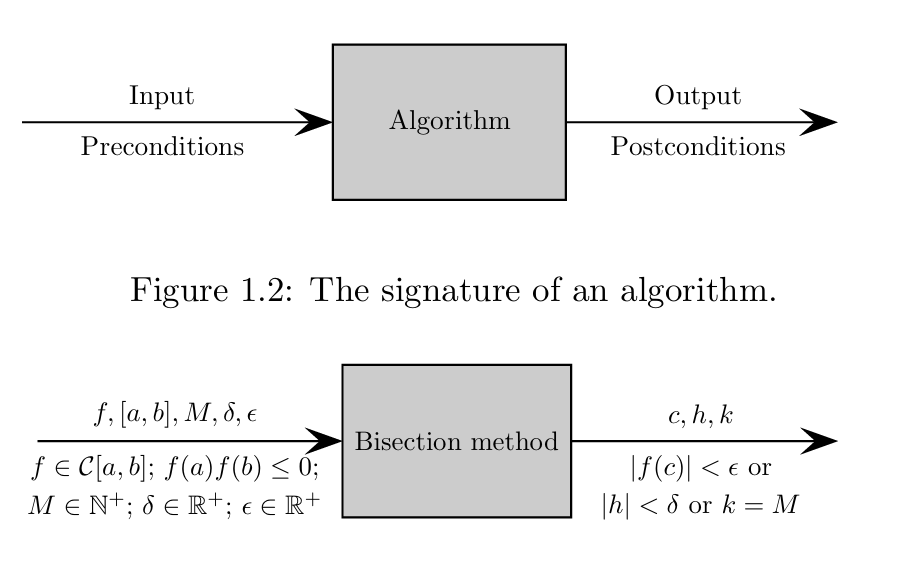
\includegraphics[width=0.75\textwidth]{images/algorithm_sign.png} % Replace with actual diagram if needed
\caption{算法的签名结构图}
\label{fig::signature}
\end{figure}

\begin{remark}
    % remark 1.3
    \label{rem::contract}
一个算法,就像一个定理,可以被看作是一个\textbf{契约(contract)}:它表示“只要你(用户)给予满足前提条件的输入,我(开发者)就会给你满足后置条件的输出。” 
一个算法可以如图~\ref{fig::signature} 所示地形式化表示。例如,二分法如图~\ref{fig::bisection} 所示。

契约,或者说断言。在定理场合,只要前提条件成立,结论就成立;在算法场合,只要输入符合前置条件,算法就会产生符合后置条件的输出。
\end{remark}

\begin{remark}
    % remark 1.4
如果先决条件被违反,算法的行为或输出将是未定义的。为了确保先决条件成立,我们可以在算法内部显式地检查它们(通常用关键字 \textbf{check} 表示),
或者将此责任转交给用户(通常用关键字 \textbf{require} 表示)。

在测试程序时,其本质是:在输入满足先决条件的测试用例后,验证后置条件是否成立。

定理需要被证明,而理论上讲,一个算法作为一个断言,也是可以被证明的,或者,作为在一个有限精度计算机上的程序,可以被测试,甚至被遍历测试。
\end{remark}

\begin{definition}
算法的签名由以下部分组成:输入、输出、前置条件、后置条件,以及对不满足前置条件的输入参数的处理方式。
\end{definition}

\begin{remark}
一个算法的签名从“黑箱”的外部唯一地决定了它的行为。
\end{remark}


\subsection{算法的正确性证明与简化}

\begin{definition}
\textbf{不变量}(invariant)是指在算法执行过程中始终成立的条件。
\end{definition}

\begin{remark}
算法的三个基本构建模块是:顺序执行的简单语句、条件语句,以及循环语句。我们特别关注的是那些在循环过程中保持不变的不变量。
\end{remark}

\begin{definition}
若某个变量在循环体内初始化,则称其为\textbf{临时变量}或\textbf{派生变量};若某个变量在进入循环之前就已初始化,并在不同迭代中保持其值的变化,
则称其为\textbf{持久变量}或\textbf{主变量}。    
\end{definition}

\begin{exercise}
算法 \ref{alg::bisection} 中的不变量有哪些?变量 \(a, b, c, h, u, v, w\) 各自表示什么?哪些是主变量?哪些是临时变量?请画出图示来说明这些变量的生命周期。    
\end{exercise}

\begin{remark}
为了证明一个算法的正确性,我们必须说明:
\begin{itemize}
  \item 算法在有限时间内终止;
  \item 输出满足后置条件。
\end{itemize}

第二点通常通过主变量的不变量,以及派生变量对主变量的依赖关系来证明。
\end{remark}

\begin{remark}
针对备注 \ref{rem::contract} 中的类比,我们关注的是黑箱的外部。事实上,该类比也适用于黑箱的内部,
含义如下:就像我们在证明定理时不需要无关或冗余的参数一样,我们也应尽可能简化算法。
\end{remark}

\begin{algorithm}
    % alg 1.9
    \label{alg::simple_bisection}
简化的二分法算法:

\begin{minipage}{0.45\textwidth}
\textbf{输入:} \\
$f : [a,b] \rightarrow \mathbb{R}$,$a \in \mathbb{R}$,$b \in \mathbb{R}$ \\
$M \in \mathbb{N}$,$\delta \in \mathbb{R}^+$,$\epsilon \in \mathbb{R}^+$ \\
\textbf{前提条件:} \\
$f \in C([a,b])$, $\text{sgn}(f(a)) \neq \text{sgn}(f(b))$ \\
\textbf{输出:} $c, h, k$ \\
\textbf{后置条件:} $|f(c)| < \epsilon$ 或 $|h| < \delta$ 或 $k = M$
\end{minipage}

\begin{enumerate}
\item $h \leftarrow b - a$
\item $u \leftarrow f(a)$
\item \textbf{for} $k = 0$ \textbf{to} $M$
\item \quad $h \leftarrow h / 2$
\item \quad $c \leftarrow a + h$
\item \quad \textbf{if} $|h| < \delta$ 或 $k = M$ \textbf{then break}
\item \quad $w \leftarrow f(c)$
\item \quad \textbf{if} $|w| < \epsilon$ \textbf{then break}
\item \quad \textbf{else if} $\text{sgn}(w) = \text{sgn}(u)$ \textbf{then}
\item \qquad $a \leftarrow c$
\item \textbf{end for}
\end{enumerate}
    
\end{algorithm}

\begin{remark}
如果将第 2 行放置在循环开始之后的位置,将更容易证明算法 \ref{alg::simple_bisection} 的正确性。
在这种情况下,证明可以基于以下两点:
\begin{enumerate}
    \item 观察到只有变量 \(a\) 是主变量,其他变量都是由 \(a\) 推导而来;
    \item 区间长度在每次迭代中都会缩小为原来的一半,这构成了一个不变量。
\end{enumerate}
此外,将第 2 行放在循环外并不会影响算法的正确性,因为在循环中我们只需要用到 \(f(a)\) 的符号。
\end{remark}

\begin{remark}
    % rem 1.10
    \label{rem::reduce_cost}
第 2 行留在循环之外的另一个重要原因是:计算非线性函数 \(f\) 可能代价较高。换句话说,我们应尽量减少在二分法循环中对 \(f\) 的求值。

事实上,只有当算法 \ref{alg::bisection} 和算法 \ref{alg::simple_bisection} 在循环中对 \(f\) 的求值次数相同,
它们在效率上才具有可比性。这也是两个算法中第 6 行的条件语句为何要与第 8 行分开的原因。
\end{remark}

\begin{remark}
算法 \ref{alg::simple_bisection} 相较于算法 \ref{alg::bisection},有哪些方面更加简单?
总的代码行数并不重要,一个更好的衡量方式是主变量的数量:算法 \ref{alg::bisection} 有四个主变量,而算法 \ref{alg::simple_bisection} 只有两个。

此外,算法 \ref{alg::simple_bisection} 中的主变量 \(h\) 是非常可预测的(在每次循环中都除以 $2$),
因此我们实际上只有一个主变量在语法结构和语义上都真正重要。
\end{remark}


\subsection{Q-阶收敛性}
% subsec 1.4
\label{subsec::Q_convergence}

\begin{definition}
    % def 1.10
    \label{def::Q_convergence}
(Q-阶收敛性)一个收敛序列 \(\{x_n\}\) 若满足以下条件,则称其以 Q-阶 \(p\)(其中 \(p \ge 1\))收敛于 \(L\):
\begin{equation}
\lim_{n \to \infty} \frac{|x_{n+1} - L|}{|x_n - L|^p} = c > 0
\end{equation}
其中常数 \(c\) 被称为\textbf{渐近因子(asymptotic factor)}。特别地:
\begin{itemize}
    \item 若 \(p = 1\),称为\textbf{线性收敛};
    \item 若 \(p = 2\),称为\textbf{二次收敛}。
\end{itemize}    
\end{definition}

\begin{remark}
收敛阶衡量的是收敛的速度。然而,只有当一个数列被证明确实收敛时,我们才能称其具有 $Q$ 阶收敛。换句话说,
定义 \ref{def::Q_convergence} 并不保证收敛,它仅仅衡量收敛的速度。

以求解 \( f(x) = \sin(x) = 0 \) 且 \( x \) 接近 $3$ 的情形为例。
如果渐近因子 \( c = 0.1 \), 那么线性收敛方法的每一次迭代将带来一位新的有效数字。如果 \( c = \frac{1}{2} \),
那么线性收敛方法的每次迭代将带来一位新的有效比特。对于二次收敛方法,每次迭代大致会使正确的数字或比特数翻倍。
\end{remark}

\begin{definition}
    % def 1.11
    \label{def::linear_convergence}
序列 \(\{x_n\}\) 若满足:
\begin{equation}
    % eq 1.2
    \label{eq::linear_convergence}
\exists c \in (0, 1), \exists d > 0, \text{使得 } \forall n \in \mathbb{N}, \quad |x_n - L| \le c^n d
\end{equation}
则称其\textbf{线性收敛于} \(L\).

若收敛序列 \(\{x_n\}\) 满足:
\begin{equation}
    % eq 1.3
    \label{eq::Q_convergence}
\exists c > 0, \exists N \in \mathbb{N}, \text{使得 } \forall n > N, \quad |x_{n+1} - L| \le c|x_n - L|^p
\end{equation}
则称其具有 \(p\) 阶收敛。  
\end{definition}

\begin{remark}
定义 \ref{def::linear_convergence} 可由定义 \ref{def::Q_convergence} 推出。(请使用定义 C.3 来证明这一点!)

请注意,(\ref{eq::linear_convergence}) 同时也保证了收敛性,而 (\ref{eq::Q_convergence}) 并不保证。例如,数列 \(\{1, -1, 1, -1, \dots\}\) 
满足 (\ref{eq::Q_convergence}) 中 \(L = 0\)、\(p = 1\)、\(c = 1\) 的条件,但该数列并不收敛。

(\ref{eq::linear_convergence}) 保证收敛性的关键在 于 \(c < 1\),而 (\ref{eq::Q_convergence}) 中的 \(c\) 可以大于 $1$.
\end{remark}

\begin{theorem}
(单调收敛定理)任何有界的单调序列都是收敛的。
\end{theorem}

\begin{theorem}
    % thm 1.13
    \label{thm::bisection}
(二分法的收敛性)设函数 \(f : [a_0, b_0] \to \mathbb{R}\) 连续,且满足 \(\text{sgn}(f(a_0)) \neq \text{sgn}(f(b_0))\),则二分法中迭代序列的误差以因子 \(\frac{1}{2}\) 线性收敛:
\begin{equation}
\lim_{n \to \infty} a_n = \lim_{n \to \infty} b_n = \lim_{n \to \infty} c_n = \alpha
\end{equation}
\begin{equation}
f(\alpha) = 0
\end{equation}
\begin{equation}
|c_n - \alpha| \le 2^{-n+1}(b_0 - a_0)
\end{equation}
其中 \([a_n, b_n]\) 表示第 \(n\) 次迭代的区间,\(c_n = \frac{1}{2}(a_n + b_n)\) 为当前迭代的中点。    
\end{theorem}

\begin{proof}
由算法定义可知:
\[
a_0 \le a_1 \le a_2 \le \cdots \le \alpha,\quad
b_0 \ge b_1 \ge b_2 \ge \cdots \ge \alpha
\]
\[
b_{n+1} - a_{n+1} = \frac{1}{2}(b_n - a_n)
\]
由单调收敛定理,\(\{a_n\}, \{b_n\}\) 均收敛,且区间长度趋于 $0$,因此中点也收敛于某个 \(\alpha\)。
由算法和初始条件可知,每次迭代区间内 \(f(a_n)f(b_n) \le 0\) 成立,故 \(f(\alpha) = 0\).
\end{proof}

\begin{remark}
请注意算法 \ref{alg::bisection} 的表示方式和循环\textit{不变量}是如何在定理 \ref{thm::bisection} 的证明中被利用的。
\end{remark}

\begin{remark}
二分法的优点包括:保证收敛、最终误差明确,并且易于并行计算。其缺点是收敛速度较慢,且在寻找满足 \( f(a)f(b) < 0 \) 的两个点 \(a, b\) 时可能存在困难。
这些观察基于一个事实:在许多实际情形中,我们可能并不知道函数 \(f(x)\) 的精确形式。
\end{remark}

\subsection{牛顿法}
\begin{remark}
    我们已经有二分法了,为何需要更多的方法?
\end{remark}

来看一个本质上快于二分法的求根算法, 因为它是 $Q$-二阶的, 而二分法是
$Q$-线性的. 它的来源是对 $f$ 在真解 $x^*$ 处做关于初值 $x_0$ 的 Taylor
展开, 并截断到第二项:
\begin{eqnarray*}
  &&0 = f(x^*)=f(x_0)+(x^* - x_0)f'(x_0) + o((x^* - x_0)^2) \\
  &\Rightarrow&f(x_0) + x^*f'(x_0) - x_0f'(x_0) \approx 0 \\
  &\Rightarrow&x^* \approx x_0 - \frac{f(x_0)}{f'(x_0)}.
\end{eqnarray*}
由此得到迭代公式.

\begin{figure}
\centering
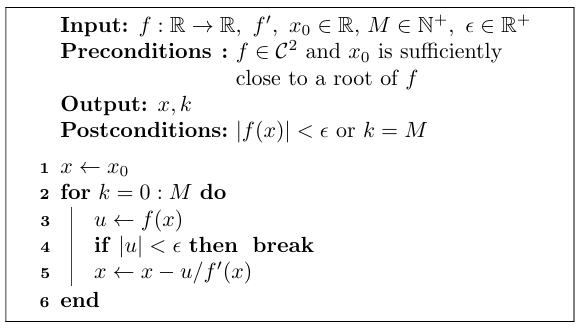
\includegraphics[width=0.75\textwidth]{images/newton_method.png}
\caption{牛顿法的步骤}    
\label{fig::newton}
\end{figure}

\begin{algorithm}
    % alg 1.14
    \label{alg::newton}
如图 \ref{fig::newton} 和 \ref{fig::geo_newton} 所示,牛顿法用于求解函数 \(f : \mathbb{R} \rightarrow \mathbb{R}\) 的根,从初始值 \(x_0\) 开始,使用迭代公式:
\begin{equation}
    % 
    \label{eq::newton}
x_{n+1} = x_n - \frac{f(x_n)}{f'(x_n)}, \quad n \in \mathbb{N}
\end{equation}
\end{algorithm}

\begin{remark}
一个函数的自变量可以包含另一个函数。这种特殊类型的函数被称为 \textit{泛函}(functional)或 \textit{函数子}(functor). 
在 \textbf{matlab} 中,函数子通过函数指针 \texttt{@} 实现;在 \textbf{C++} 中,函数子是具有 \texttt{operator()} 的类。
\end{remark}

\begin{remark}
牛顿法收敛得非常快,以至于在二分法中所需的停止准则 \(\delta\) 并不是必须的。
\end{remark}

\begin{figure}
\centering
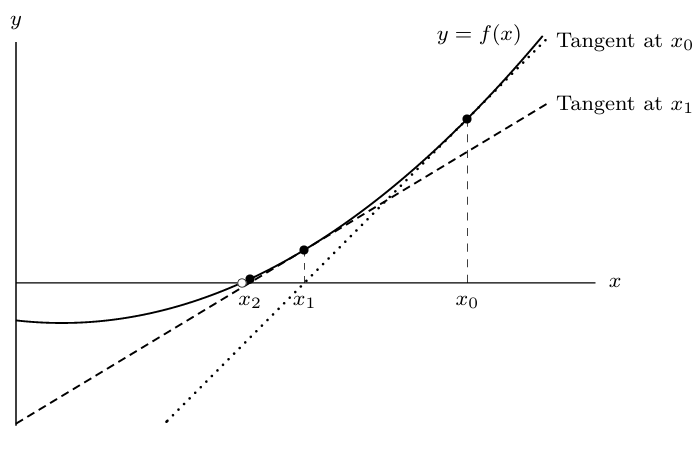
\includegraphics[width=0.75\textwidth]{images/geo_newton.png}
\caption{牛顿法的几何解释}
\label{fig::geo_newton}
\end{figure}

\begin{theorem}
    % 1.15
    \label{thm::newton}
(牛顿法的收敛性)  
设 \( f : \mathcal{B} \to \mathbb{R} \) 是定义在区间 \( \mathcal{B} = [\alpha - \delta, \alpha + \delta] \) 上的 \( C^2 \) 函数,
满足 \( f(\alpha) = 0 \) 且 \( f'(\alpha) \ne 0 \). 
若初始点 \( x_0 \) 足够接近根 \(\alpha\),则牛顿法生成的迭代序列 \(\{x_n\}\) 至少以\textbf{二次速度}收敛于 \(\alpha\),即:
\begin{equation}
\lim_{n \to \infty} \frac{\alpha - x_{n+1}}{(\alpha - x_n)^2} = \frac{f''(\alpha)}{2f'(\alpha)}.     
\end{equation}    
\end{theorem}

\begin{proof}
由泰勒公式(定理 C.99)和 \(f \in C^2\) 得:
\[
f(\alpha) = f(x_n) + (\alpha - x_n) f'(x_n) + \frac{(\alpha - x_n)^2}{2} f''(\xi)
\]
其中 \(\xi\) 在 \(x_n\) 与 \(\alpha\) 之间。因为 \(f(\alpha) = 0\),代入得:
\[
- \alpha = - x_n - \frac{f(x_n)}{f'(x_n)} + \frac{(\alpha - x_n)^2}{2} \frac{f''(\xi)}{f'(x_n)}
\]
即:
\[
x_{n+1} - \alpha = (x_n - \alpha)^2 \cdot \frac{f''(\xi)}{2f'(x_n)} \tag{*}
\]
由 \(f'(\alpha) \ne 0\) 的连续性可知,存在 \(\delta_1, \delta_2 > 0\),使得在集合 \(B_1 = [\alpha - \delta_1, \alpha + \delta_1]\) 中,\(f'(x)\) 有界且不为零。
设:
\[
M := \frac{\max_{x \in B_1} |f''(x)|}{2 \min_{x \in B_1} |f'(x)|}
\]
若初始点 \(x_0\) 满足:
\begin{itemize}
    \item[(i)] \(|x_0 - \alpha| = \delta_0 < \delta_1\);
    \item[(ii)] \(M \delta_0 < 1\).
\end{itemize}
则根据 (*) 式可得:
\[
|x_{n+1} - \alpha| \le M |x_n - \alpha|^2
\]
所以收敛阶为 $2$. 并且由归纳法可得:
\[
|x_n - \alpha| \le \frac{1}{M} (M |x_0 - \alpha|)^{2^n}
\]
这证明了二次收敛性。若 \(f''(\alpha) = 0\),收敛速率可能高于二次。 
\end{proof}

\begin{remark}
短语 “至少”(at least)指的是超收敛情形,即 \( f''(\alpha) = 0 \). 
定理 \ref{thm::newton} 中模糊的表达 “足够接近”(sufficiently close)指的是其证明中条件 (i)、(ii),这两个条件必须同时满足。

换句话说,我们并没有一个逐步构造 \( x_0 \) 来满足这些条件的方法;我们甚至不会去尝试。
为什么?因为我们对函数 \( f \) 的信息不足。我们所能做的最好的事情,就是要求条件 (i)、(ii) 同时成立。
\end{remark}

\begin{remark}
牛顿法的主要优点是其收敛速度非常快。其缺点之一是需要我们知道导数 \( f'(x) \), 
而这可能难以获得,或者计算起来耗时较长。牛顿法的另一个主要缺点是我们无法判断初始点 \( x_0 \) 是否足够接近真实根。因此,收敛性无法得到保证。

例如,如果在定理 \ref{thm::newton} 的证明中条件 (i) 被违反,那么下一次迭代可能会远离根 \(\alpha\). 图 \ref{fig::newton_cond} 展示了条件 (ii) 的必要性。
\end{remark}

\begin{figure}
    % fig 1.6
    \label{fig::newton_cond}
\centering
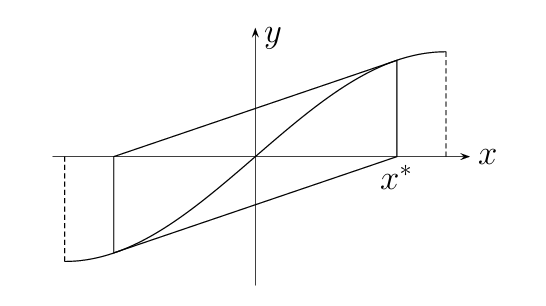
\includegraphics[width=0.5\textwidth]{images/newton_cond.png} % Replace with actual image
\caption{展示定理 \ref{thm::newton} 中条件必要性的特殊例子}
\end{figure}

\begin{theorem}
    % 1.16
    \label{thm::monotone}
若连续函数 \(f: [a,b] \to [c,d]\) 是双射,当且仅当 \(f\) 是严格单调的。
\end{theorem}

\begin{remark}
定理 \ref{thm::monotone} 的充分性部分可以重述为:“如果函数 \( f : [a, b] \to [c, d] \) 是连续且严格单调的,那么它是双射(bijective)。”\\
但其逆命题并不成立。你能给出一个反例吗?
\end{remark}

\begin{remark}
我们注意到,由于缺乏对函数 \( f \) 的信息,牛顿法的收敛性无法得到保证。解决该问题的一种方法是对 \( f \) 施加更多条件;定理 \ref{thm::newton_monotone} 就是一个例子。
\end{remark}

\begin{theorem}
    % thm 1.17
    \label{thm::newton_monotone}    
若 \(f : \mathbb{R} \to \mathbb{R}\) 为 \(C^2\) 函数,满足:
\begin{itemize}
    \item \(f(\alpha) = 0\)
    \item \(f' > 0\), \(f'' > 0\)
    \item \(\alpha\) 是 \(f\) 的唯一根
\end{itemize}
则对于任意 \(x_0 > \alpha\), 牛顿法迭代序列 \(\{x_n\}\) 二次收敛于 \(\alpha\).    
\end{theorem}

\begin{proof}
由定理 \ref{thm::monotone} 可知,函数 \( f \) 是双射,因为 \( f \) 是连续且严格单调的。
由于 \( 0 \) 在其值域中,\( f \) 必有唯一根。在证明定理 \ref{thm::newton} 时,我们有:

\begin{equation}
    % eq 1.9
    \label{eq::newton_residual}
x_{n+1} - \alpha = (x_n - \alpha)^2 \cdot \frac{f''(\xi)}{2 f'(x_n)}. 
\end{equation}

进一步地,\( f' > 0 \) 且 \( f'' > 0 \) 意味着对所有 \( n > 0 \), 
都有 \( x_n > \alpha \). 由于 \( f \) 是严格递增的,意味着 \( f(x_n) > f(\alpha) = 0 \), 
对所有 \( n > 0 \) 成立。根据牛顿法的定义,

\[
x_{n+1} - \alpha = x_n - \alpha - \frac{f(x_n)}{f'(x_n)},
\]

因此序列 \( \{x_n - \alpha : n > 0\} \) 是严格单调递减的,且以 $0$ 为下界。
由定理 \ref{eq::secant} 可知,该序列收敛。

设 \( \lim_{n \to \infty} x_n = a \),两边对等式 (\ref{eq::newton}) 取极限得:

\[
a = a - \frac{f(a)}{f'(a)},
\]

由此可得 \( f(a) = 0 \). 由于 \( f \) 的根是唯一的,因此 \( a = \alpha \)。

二次收敛速率可使用等式 (\ref{eq::newton_residual}) 进行归纳证明,如同在定理 \ref{thm::newton} 中所做的那样。
\end{proof}

\begin{remark}
对牛顿迭代 \( (x_n)_{n \in \mathbb{N}} \) 唯一收敛于 \(\alpha\) 的证明如下。

假设数列 \(\{x_n\}\) 收敛于 \(\alpha + c\),其中 \(c > 0\) 为某个固定常数。定义:
\[
\delta = \frac{f(\alpha + c)}{f'(\alpha + c)}.
\]
将 \(f(\alpha + c)\) 在 \(\alpha\) 处展开为泰勒级数,结合 \(f'(\alpha + c) > 0\) 可知 \(\delta > 0\)。因为牛顿迭代 \(\{x_n\}\) 收敛,所以有:
\[
\forall \epsilon > 0,\ \exists N \in \mathbb{N},\ \text{使得} \ \forall n > N,\ |x_n - x_{n+1}| = \left| \frac{f(x_n)}{f'(x_n)} \right| < \epsilon,
\]
尤其当 \(\epsilon = \frac{1}{2} \delta\) 时成立。

另一方面,
\[
\left| x_n - x_{n+1} - \frac{f(\alpha + c)}{f'(\alpha + c)} \right|
\geq \left| x_n - x_{n+1} \right| - \left| \frac{f(\alpha + c)}{f'(\alpha + c)} \right|
> \delta - \frac{1}{2} \delta = \frac{1}{2} \delta = \epsilon.
\]

这与牛顿迭代 \(\{x_n\}\) 收敛于 \(\alpha + c\) 的假设矛盾。因此结合前面的推理,说明牛顿迭代 \(\{x_n\}\) 实际上收敛于 \(\alpha\),即 \(f\) 的唯一根。
\end{remark}

\begin{definition}
向量空间 \(V\) 的子集 \(\mathcal{U}\) 是凸集当且仅当:
\begin{equation}
\forall x, y \in \mathcal{U}, \forall t \in (0,1), \quad tx + (1 - t)y \in \mathcal{U} 
\end{equation}
即线段上的所有点都在集合中。    
\end{definition}

\begin{definition}
函数 \(f : \mathcal{U} \to \mathbb{R}\) 是凸函数当且仅当:

\begin{equation}
    % eq 1.11
    \label{eq::convex_function}
\forall x, y \in \mathcal{U}, \forall t \in (0,1), \quad f(tx + (1 - t)y) \le t f(x) + (1 - t) f(y) 
\end{equation}    
\end{definition}

若将 \ref{eq::convex_function} 中“\(\le\)”换为“\(<\)”,则称 \(f\) 为严格凸函数。


\begin{remark}
一个 \( C^2 \) 函数 \( f : I \to \mathbb{R} \) 是凸的,当且仅当 \( f'' \geq 0 \) 在区间 \( I \) 上成立。
我们现在可以看到,定理 \ref{thm::newton_monotone} 中对函数 \( f \) 的要求是严格单调性和严格凸性。
\end{remark}

\begin{remark}
牛顿法可以通过反函数定理 D.120 直接推广到非线性方程组的情形;参见备注 D.53。
\end{remark}

\subsection{割线法}

\begin{remark}
如前所述,计算导数 \( f'(x) \) 可能代价非常高。为了降低计算成本,我们可以重复利用 \( x_n \) 和 \( x_{n-1} \) 处的函数值来近似导数。
这正是弦截法(secant method)的核心思想,它通常具有较高的性价比。
\end{remark}

\begin{algorithm}
如图~\ref{fig::secant-alg} 所示,割线法用于在初始猜测 \( x_0, x_1 \) 附近求解函数 \( f : \mathbb{R} \to \mathbb{R} \) 的根,其迭代公式为:
\begin{equation}
    % eq 1.12
    \label{eq::secant}
x_{n+1} = x_n - f(x_n) \frac{x_n - x_{n-1}}{f(x_n) - f(x_{n-1})}, \quad n \in \mathbb{N}^+.
\end{equation}
    
\end{algorithm}

\begin{figure}
\centering
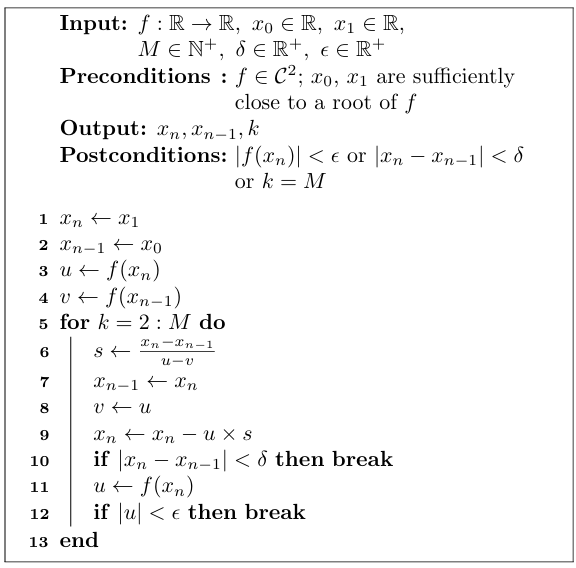
\includegraphics[width=0.75\textwidth]{images/secant_method.png} % 替换为实际图像
\caption{割线法算法}
\label{fig::secant-alg}
\end{figure}

\begin{remark}
我们将第 10 行的条件判断与第 12 行的分开,以减少对非线性函数的求值次数;参见备注 \ref{rem::reduce_cost}。
\end{remark}

\begin{definition}
    % 1.21
    \label{def::fibonacci}
斐波那契数列 \( \{F_n\} \) 定义为:
\begin{equation}
    % eq 1.13
    \label{eq::fibonacci}
F_0 = 0, \quad F_1 = 1, \quad F_{n+1} = F_n + F_{n-1}.
\end{equation}
\end{definition}

\begin{theorem}[Binet 公式]
    % 1.22
    \label{thm::binet}
设黄金比例为 \( r_0 = \frac{1+\sqrt{5}}{2} \),其共轭根为 \( r_1 = 1 - r_0 = \frac{1 - \sqrt{5}}{2} \),则斐波那契数列可表示为:
\begin{equation}
    % eq 1.14
F_n = \frac{r_0^n - r_1^n}{\sqrt{5}}.
\end{equation}
\end{theorem}

\begin{proof}
由定义 \ref{def::fibonacci} 可得:

令
\[
\mathbf{u}_k := 
\begin{bmatrix}
F_{k+1} \\
F_k
\end{bmatrix},
\quad
A := 
\begin{bmatrix}
1 & 1 \\
1 & 0
\end{bmatrix},
\]
则有 \( \mathbf{u}_k = A^k \mathbf{u}_0 \)。因此特征方程为:
\[
\det(A - \lambda I) = \lambda^2 - \lambda - 1 = 0
\]
其根为 \( r_0, r_1 \)。设对应特征向量为 \( \mathbf{x}_0, \mathbf{x}_1 \),则
\[
\mathbf{u}_0 = \frac{1}{r_0 - r_1} (r_0 \mathbf{x}_0 - r_1 \mathbf{x}_1)
\]
代入得结果。
\end{proof}

\begin{remark}
由于 \( r_0 \approx 1.618 \), \( r_1 \approx -0.618 \), 我们有
\[
\lim_{n \to +\infty} \left(F_n - \frac{r_0^n}{\sqrt{5}}\right) = 0.
\]
为了用浮点数计算 \( F_n \), 可以先计算 \( r_0^n / \sqrt{5} \), 再将结果四舍五入为最接近的整数以得到 \( F_n \). 
然而,这种方法可能比直接使用公式 (\ref{eq::fibonacci}) 计算慢得多。为什么?
\end{remark}

\begin{corollary}
    % 1.23
    \label{cor::fib_recurrence}
定理 \ref{thm::binet} 中的 \( r_0, r_1 \) 满足:
\begin{equation}
    % eq 1.15
F_{n+1} = r_0 F_n + r_1^n.
\end{equation}
\end{corollary}

\begin{lemma}[割线法误差表达式]
    % 1.24
    \label{lem::secant_error}
对于割线法(\ref{eq::secant}),存在 \( \xi_n \in (x_{n-1}, x_n) \), 
\( \zeta_n \in \big( \min(x_{n-1}, x_n, \alpha), \max(x_{n-1}, x_n, \alpha) \big) \), 使得:
\begin{equation}
    % eq 1.16
x_{n+1} - \alpha = (x_n - \alpha)(x_{n-1} - \alpha) \cdot \frac{f''(\zeta_n)}{2 f'(\xi_n)}.
\end{equation}
\end{lemma}

\begin{proof}
定义割差为:
\begin{equation}
    % eq 1.17
f[a,b] = \frac{f(a) - f(b)}{a - b}.
\end{equation}

代数变换可得公式等价为:
\begin{equation}
    % eq 1.18
x_{n+1} - \alpha = (x_n - \alpha)(x_{n-1} - \alpha) \cdot \frac{f[x_n, x_{n-1}] - f[x_n, \alpha]}{f[x_{n-1}, x_n]}.
\end{equation}

由平均值定理存在 \( \xi_n \in (x_{n-1}, x_n) \) 使得:
\begin{equation}
    % eq 1.19
f[x_{n-1}, x_n] = f'(\xi_n)
\end{equation}

定义 \( g(x) := f[x, x_n] \),再应用平均值定理,有:
\begin{equation}
    % eq 1.20
\frac{f[x_n, x_{n-1}] - f[x_n, \alpha]}{x_{n-1} - \alpha} = g'(\beta)
\end{equation}

对 \( g'(x) \) 求导并使用拉格朗日余项公式,有:
\begin{equation}
    % eq 1.21
\frac{f[x_n, x_{n-1}] - f[x_n, \alpha]}{x_{n-1} - \alpha} = \frac{f''(\zeta_n)}{2}
\end{equation}
代入即得结论。
\end{proof}

\begin{theorem}[割线法收敛性]
    % 1.25
    \label{thm::secant}
设函数 \( f : \mathcal{B} \to \mathbb{R} \) 为 \( C^2 \) 函数,
定义在区间 \( \mathcal{B} = [\alpha - \delta, \alpha + \delta] \) 上,
满足 \( f(\alpha) = 0 \)、\( f'(\alpha) \ne 0 \)、\( f''(\alpha) \ne 0 \),
若初始点 \( x_0, x_1 \) 足够接近 \(\alpha\),则割线法迭代序列 \( \{x_n\} \) 收敛于 \(\alpha\),其收敛阶为:
\begin{equation*}
    \label{eq::golden_ratio}
p = \frac{1 + \sqrt{5}}{2} \approx 1.618.
\end{equation*}
\end{theorem}

\begin{proof}
由于 \( f' \) 连续,且 \( f'(\alpha) \ne 0 \),可得存在 \( \delta_1 > 0 \),使得对所有 \( x \in B_1 \subseteq \mathcal{B} \),有 \( f'(x) \ne 0 \).

设 \( B_1 = [\alpha - \delta_1, \alpha + \delta_1] \),定义 \( E_i = |x_i - \alpha| \),
\[
M = \frac{\displaystyle \max_{x \in B_1} |f''(x)|}{\displaystyle 2 \min_{x \in B_1} |f'(x)|}
\]
由引理 \ref{lem::secant_error} 可得:
\begin{equation*}
ME_{n+1} \leq ME_n ME_{n-1}.
\end{equation*}

选择初始点 \(x_0, x_1\) 满足:

\begin{enumerate}
    \item \( E_0 < \delta, \quad E_1 < \delta \);
    \item \( \max(ME_1, ME_0) = \eta < 1 \).
\end{enumerate}

则根据上述递推关系,可由归纳法证明:存在 \(\eta\) 使得所有 \( ME_n < \eta \)。记 \( ME_0 \leq \eta \),
 \( ME_1 \leq \eta \), 
 \( ME_2 \leq ME_1 ME_0 \leq \eta^2 \), 以此类推,得:
\[
E_n \leq B_n := \frac{1}{M} \eta^n,
\]
其中 \( \{q_n\} \) 是从 \( q_0 = 1, q_1 = 1 \) 开始的斐波那契数列。由定理 \ref{eq::golden_ratio} 可得:
\[
q_n \sim \frac{1.618^{n+1}}{\sqrt{5}},
\]
从而 \( \lim_{n \to \infty} E_n = 0 \).

为了估计收敛速率,首先研究上界 \( \{B_n\} \) 的下降速度:

\begin{equation*}
\frac{B_{n+1}}{E_0^\eta} = \left( \frac{1}{M} \right)^\eta \eta^{q_{n+1}} = M^{r_0 - 1} \eta^{-r_1 - r_0 q_n} \leq M^{r_0 - 1} \eta^{-1},
\end{equation*}

其中 \( q_{n+1} - r_0 q_n = r_1^{n+1} \to -1 \)。

为证明收敛速率,我们定义:
\begin{equation}
    % eq 1.22
m_n := \frac{f''(\zeta_n)}{2f'(\xi_n)}, \quad m_\alpha := \left| \frac{f''(\alpha)}{2f'(\alpha)} \right|,
\end{equation}

其中 \( \zeta_n, \xi_n \) 与引理 \ref{lem::secant_error} 中相同。

通过归纳法,我们有:
\begin{align*}
E_n &= E_1^{{F_n}} E_0^{{F_{n-1}}} m_1^{F_{n-1}} \cdots m_{n-1}^{F_1}, \\
E_{n+1} &= E_1^{F_{n+1}} E_0^{F_n} m_1^{F_n} \cdots m_n^{F_1},
\end{align*}

其中 \( F_n \) 是定义 \ref{def::fibonacci} 中的斐波那契数列。于是,

\begin{equation}
    % eq 1.23
    \begin{array}{rcl}
\frac{E_{n+1}}{E_0^{F_n}} &=& E_1^{F_{n+1} - r_0 F_n} E_0^{F_n - r_0 F_{n-1}} m_1^{F_n - r_0 F_{n-1}} \cdots m_n^{F_1 - r_0 F_0}, \\
&=& E_1^{F_{n+1} - r_0 F_n} E_0^{F_n - r_0 F_{n-1}} \prod_{j=1}^n m_j^{F_{n+1-j} - r_0 F_{n-j}}, \\
&=& E_1^{r_1^{n-1}} E_0^{r_1^{n-2}} \cdots m_1^{r_1^1} m_n^{r_1^n}.
    \end{array}
\end{equation}

由推论 \ref{cor::fib_recurrence} 可得:

% \begin{equation}
%     % eq 1.24
% \lim_{n \to \infty} \frac{E_{n+1}}{E_0^{F_n}} = \lim_{n \to \infty} A \cdot \lim_{n \to \infty} B 
% = \lim_{n \to \infty} B \leq 2^{r_1 + r_1^2 + \cdots} \cdot \frac{1}{m_\alpha^0}.
% \end{equation}

\begin{equation}
    % eq 1.24
\lim_{n \to \infty} m_n = m_\alpha,
\end{equation}

于是存在常数 \( N \in \mathbb{N} \),使得对所有 \( n > N \),有:
\begin{equation}
    % eq 1.25
m_n \in \left( \frac{1}{2} m_\alpha, 2m_\alpha \right)
\end{equation}

定义:
\begin{equation*}
A := E_1^{r_1^{n-1}} E_0^{r_1^{n-2}} \cdots m_1^{r_1^1} m_2^{r_1^2} \cdots m_{N}^{r_1^N}
\end{equation*}

\begin{equation*}
B := m_{N+1}^{r_1^{N+1}} \cdots m_n^{r_1^n}
\end{equation*}

因此:
\begin{equation*}
\lim_{n \to \infty} B \leq 2^{\sum_{i=N+1}^{\infty} r_1^i} \cdot \frac{1}{m_\alpha^0}
\end{equation*}
\end{proof}

\begin{remark}
尽管牛顿法具有更高的收敛速度,弦截法可能计算代价更低。因此,对于一个给定的问题,我们应如何在牛顿法和弦截法之间做出选择?
如果我们 \textit{事先} 知道所需解的精度,那就选择 \textbf{CPU 时间更少} 的方法。
\end{remark}

\begin{corollary}
    % 1.26
    \label{cor::newton_secant_time}
若考虑 \( f(x) = 0 \) 在 \( x = \alpha \) 处的根,记 \( m \) 和 \( sm \) 分别为评估 \( f(x) \) 与 \( f'(x) \) 所需的时间,则达到所需精度所需的最短迭代次数分别为:

\begin{equation}
    % eq 1.26
    \label{eq::newton_secant_time}
T_N = (1 + s)m \lceil \log_2 K \rceil,
\end{equation}

\begin{equation}
    % eq 1.27
T_S = m \lceil \log_{r_0} K \rceil + m,
\end{equation}

其中:
\begin{equation*}
r_0 = \frac{1 + \sqrt{5}}{2}, \quad c = \left| \frac{f''(\alpha)}{2f'(\alpha)} \right|,
\end{equation*}

\begin{equation}
    % eq 1.28
K = \frac{\log c}{\log |x_0 - \alpha|},
\end{equation}

符号 \( \lceil \cdot \rceil \) 表示向上取整。
\end{corollary}

\begin{proof}
在定理 \ref{thm::newton} 中我们已证明 \( |x_n - \alpha| \leq \frac{1}{M} (ME_0)^{2^n} \), 令 \( E_n = |x_n - \alpha| \), 则有:
\[
ME_n \leq (ME_0)^{2^n}
\]

设 \( i \in \mathbb{N} \) 为最小次数使得误差满足 \( (ME_0)^{2^i} \leq M\epsilon \). 当 \( \epsilon \) 足够小时,\( M \to c \), 因此:

\[
i = \lceil \log_2 K \rceil
\]

对于牛顿法,每轮迭代需要一次函数和导函数评估,总耗时 \( (1 + s)m \). 因此有公式 (\ref{eq::newton_secant_time})。

对于割线法,假设 \( ME_0 \geq ME_1 \)。由定理 \ref{thm::secant} 可得:

\[
ME_n \approx (ME_0)^{\frac{\sqrt{5}}{2} r_0^{n+1}}
\]

忽略指数中的 \( -\frac{\sqrt{5}}{2} r_1^{n+1} \) 项。设 \( j \in \mathbb{N} \) 为最小迭代次数使得误差满足 \( r_0^{\sqrt{5} j} \leq K \), 因此:

\[
j = \left\lceil \frac{\log_{r_0} K + \log_{r_0} \sqrt{5}}{\sqrt{5}} \right\rceil = \lceil \log_{r_0} K \rceil + 1.
\]

由于割线法中初始值 \(x_0\) 和 \(x_1\) 已给出,因此最少迭代次数为 \(\lceil \log_{r_0} K \rceil\)(可与牛顿法比较!)。
此外,由于前一次迭代中已计算 \(f(x_{n-1})\),因此每次迭代仅需计算函数值 \(f(x_n)\)。最后,额外的项 \(m\) 是因为在第一次迭代中还需要计算 \(f(x_0)\).
\end{proof}

\begin{remark}
根据推论 \ref{cor::newton_secant_time},当比值 \( T_S / T_N < 1 \) 时,弦截法比牛顿法更快。这意味着
\[
s > \frac{\log 2}{\log r_0} - 1 \approx 0.44.
\]
\end{remark}

\subsection{不动点迭代}
% subsec 1.7

\begin{definition}
    % 1.27
一个函数 \( g \) 的\textbf{不动点} 是满足 \( g(\alpha) = \alpha \) 的自变量 \(\alpha\).
\end{definition}

\begin{example}
    % 1.28
函数 \( f(x) = x^2 - 3x + 4 \) 的不动点是 \( x = 2 \).
\end{example}

\begin{remark}
对于函数 \( f \) 的一个不动点,我们有
\[
f^n(x) := f(f(\cdots f(x))) = x,
\]
对任意 \( n \in \mathbb{N}^+ \) 成立。因此,这个名称由此而来。
\end{remark}

\begin{lemma}
    % 1.29
    \label{lem::fixed_point}
若 \( g : [a, b] \to [a, b] \) 连续,则 \( g \) 至少在区间 \([a, b]\) 上有一个不动点。
\end{lemma}

\begin{proof}
函数 \( f(x) = g(x) - x \) 满足 \( f(a) \geq 0 \)、\( f(b) \leq 0 \),由介值定理得证。
\end{proof}

\begin{exercise}
    % 1.30
    \label{exe::no_fixed_point}
设 \( A = [-1, 0) \cup (0, 1] \). 给出一个连续函数 \( g : A \to A \), 使其没有不动点。
再给出一个从 \( \mathbb{R} \to \mathbb{R} \) 的连续函数,其同样没有不动点。
\end{exercise}

\begin{remark}
引理 \ref{lem::fixed_point} 和习题 \ref{exe::no_fixed_point} 表明:若一个连续函数的定义域和值域是相同的集合 \( A \), 
在 \( A \) 满足某些条件时,该函数就会有不动点。那么,这些条件是什么呢?布劳威尔不动点定理为我们提供了一些线索。
\end{remark}

\begin{theorem}[Brouwer 不动点定理]
    % 1.31
    \label{thm::brouwer}
设 \( \mathbb{D}^n := \{ x \in \mathbb{R}^n : \|x\| \leq 1 \} \), 则任意连续函数 \( f : \mathbb{D}^n \to \mathbb{D}^n \) 至少有一个不动点。
\end{theorem}

\begin{proof}
见 Milnor [1978]。
\end{proof}

\begin{example}
    % 1.32
将一张地图放在地板上,设函数将地图上的每个点映射到其在地图上的对应位置。若地图是 \( \mathbb{D}^2 \) 的同胚映射,则存在某个点刚好映射到其在地面上的位置。
\end{example}

\begin{exercise}
    % 1.33
将两张相同大小的纸重叠放置,然后揉皱上面的一张纸并压在下面的一张上,证明至少存在一个点在揉皱后仍位于原处。
\end{exercise}

\begin{definition}
    % 1.34
\textbf{不动点迭代} 是通过如下形式迭代寻找不动点的方法:
\begin{equation}
    % eq 1.10
x_{n+1} = g(x_n), \quad n \in \mathbb{N}.
\end{equation}
\end{definition}

\begin{example}
    % 1.35
牛顿法就是一种不动点迭代。
\end{example}

\begin{exercise}
    % 1.36
    \label{exe::fixed_point_behavior}
设 \( f(x) = x^2 - a \), 求平方根问题可转化为寻找不动点的问题。对于 \( a = 1 \), 考虑如下三种迭代函数:
\begin{itemize}
    \item \( g_1(x) = \frac{1}{2}(x + \frac{a}{x}) \)(收敛)
    \item \( g_2(x) = x^2 + a \)(发散)
    \item \( g_3(x) = \frac{1}{2}(x + a) \)(振荡)
\end{itemize}
解释这些行为。
\end{exercise}

\begin{definition}
    % 1.37
若函数 \( f : [a, b] \to [a, b] \) 存在 \( \lambda \in [0, 1) \) 使得对任意 \( x, y \in [a, b] \) 有:
\begin{equation}
|f(x) - f(y)| \leq \lambda |x - y|,
\end{equation}
则称 \( f \) 为\textbf{压缩映射(contraction mapping)}。
\end{definition}

\begin{example}
    % 1.38
任意线性函数 \( f(x) = \lambda x + c \),其中 \( 0 \leq \lambda < 1 \),是压缩映射。
\end{example}

\begin{theorem}[压缩映射收敛定理]
    % 1.39
    \label{thm::contraction}
若 \( g(x) \) 是区间 \([a, b]\) 上的压缩映射,则它在 \([a, b]\) 内有唯一的不动点 \( \alpha \). 并且,迭代公式
\[
x_{n+1} = g(x_n)
\]
对于任意初始值 \( x_0 \in [a, b] \) 都收敛于 \( \alpha \),且有误差估计:
\begin{equation}
|x_n - \alpha| \leq \frac{\lambda^n}{1 - \lambda} |x_1 - x_0|.
\end{equation}
\end{theorem}

\begin{proof}
由引理 \ref{lem::fixed_point},存在至少一个不动点。若存在两个不动点 \( \alpha, \beta \), 则:
\[
|\alpha - \beta| = |g(\alpha) - g(\beta)| \leq \lambda |\alpha - \beta| < |\alpha - \beta|
\]
矛盾,故不动点唯一。

由定义有:
\[
|x_{n+1} - \alpha| = |g(x_n) - g(\alpha)| \leq \lambda |x_n - \alpha|
\]
归纳得:
\[
|x_n - \alpha| \leq \lambda^n |x_0 - \alpha|
\]
三角不等式推导可得误差估计。
\end{proof}

\begin{remark}
定理 \ref{thm::contraction} 不应与定理 \ref{thm::brouwer} 混淆。关于定理 \ref{thm::contraction} 的一个部分推广,可参见定理 D.118。
\end{remark}

\begin{remark}
有时判断一个函数是否为压缩映射是困难的。另一种方法是检查该函数的导数的绝对值是否 \textbf{处处小于 $1$}.
\end{remark}

\begin{theorem}
    % 1.40
    \label{thm::fixed_point_convergence}
设 \( g : [a, b] \to [a, b] \), 且 \( g \in C^1[a, b] \), 记
\[
\lambda = \max_{x \in [a, b]} |g'(x)| < 1,
\]
则 \( g \) 在 \([a, b]\) 上有唯一不动点 \(\alpha\),且迭代
\[
x_{n+1} = g(x_n)
\]
收敛于 \(\alpha\), 误差估计同理成立,同时:
\begin{equation}
\lim_{n \to \infty} \frac{x_{n+1} - \alpha}{x_n - \alpha} = g'(\alpha).
\end{equation}
\end{theorem}

\begin{proof}
由均值定理 \( g(x_n) - g(\alpha) = g'(\xi)(x_n - \alpha) \), 其中 \( \xi \in (x_n, \alpha) \). 取极限,得结论。
\end{proof}

\begin{corollary}
    % 1.41
    \label{cor::fixed_point_derivative}
设 \( \alpha \) 是函数 \( g : \mathbb{R} \to \mathbb{R} \) 的不动点,
\( g \in C^1(B_0) \), 其中 \( B_0 = [\alpha - \delta, \alpha + \delta] \), 若 \( |g'(\alpha)| < 1 \), 则:

存在 \( \delta_0 > 0 \), 使得若 \( x_0 \in B_0 \) 且 \( \max_{x \in B_0} |g'(x)| < 1 \), 则定理 \ref{thm::contraction} 成立。
\end{corollary}

\begin{proof}
选择 \( \lambda \in (|g'(\alpha)|, 1) \), 选取 \( \delta_0 \) 使得 \( g \) 在 \( B_0 \subseteq [\alpha - \delta_0, \alpha + \delta_0] \) 
上满足 \( |g'(x)| \leq \lambda \), 由定理 \ref{thm::fixed_point_convergence} 得证。
\end{proof}

\begin{remark}
此时正是回到习题 \ref{exe::fixed_point_behavior} 并解释这三种方法的不同行为的好时机。
\end{remark}



\begin{corollary}
    % 1.42
    \label{cor::fixed_point_higher_order}
设函数 \( g : [a, b] \to [a, b] \) 有不动点 \( g(\alpha) = \alpha \in [a, b] \). 若不动点迭代
\begin{equation}
    % eq 1.29
x_{n+1} = g(x_n)
\end{equation}
以 \( p \) 阶精度(其中 \( p > 1,\, p \in \mathbb{N} \))收敛于 \(\alpha\),则需满足:

\begin{equation}
    % eq 1.30
\left\{
\begin{aligned}
&g \in C^p[a, b], \\
&\forall k = 1, 2, \ldots, p - 1,\quad g^{(k)}(\alpha) = 0, \\
&g^{(p)}(\alpha) \ne 0
\end{aligned}
\right.
\end{equation}

且初始点 \( x_0 \) 足够接近 \(\alpha\).
\end{corollary}

\begin{proof}
由推论 \ref{cor::fixed_point_derivative} 可知 \( g'(\alpha) = 0 \), 又由于 \( g' \) 连续,存在 \( \delta > 0 \), 
使得不动点迭代在区间 \( [\alpha - \delta, \alpha + \delta] \) 内唯一收敛至 \(\alpha\).

由 \( g \) 在 \(\alpha\) 处的泰勒展开,有:
\begin{equation*}
\begin{array}{rcl}
    E_{\text{abs}}(x_{n+1}) &:=& |x_{n+1} - \alpha| = |g(x_n) - g(\alpha)| \\
&=& \left| \sum_{i=1}^{p-1} \frac{(x_n - \alpha)^i}{i!} g^{(i)}(\alpha) + \frac{(x_n - \alpha)^p}{p!} g^{(p)}(\xi) \right|
\end{array}
\end{equation*}
其中 \( \xi \in [a, b] \). 由于 \( g^{(p)} \) 在 \([a, b]\) 上连续,根据定理 C.70,可得其有界。因此存在常数 \( M \), 使得
\begin{equation}
E_{\text{abs}}(x_{n+1}) < M E_{\text{abs}}^p(x_n).
\end{equation}
\end{proof}

\begin{example}
    % 1.43
下列方法具有三阶收敛性,用于计算 \( \sqrt{R} \):
\begin{equation}
x_{n+1} = \frac{x_n (x_n^2 + 3R)}{3x_n^2 + R}
\end{equation}

首先,\( \sqrt{R} \) 是函数
\begin{equation}
F(x) = \frac{x(x^2 + 3R)}{3x^2 + R}
\end{equation}
的不动点。

验证:
\begin{equation}
F(\sqrt{R}) = \frac{\sqrt{R}(R + 3R)}{3R + R} = \sqrt{R}
\end{equation}

其次,\( F(x) \) 的导数如下表:

\begin{table}
\centering
\caption{函数 \( F(x) \) 的导数}
\begin{tabular}{@{}c|c|c@{}}
\toprule
\( n \) & \( F^{(n)}(x) \) & \( F^{(n)}(\sqrt{R}) \) \\
\midrule
1 & \( \dfrac{3(x^2 - R)^2}{(3x^2 + R)^2} \) & 0 \\
2 & \( \dfrac{48Rx(x^2 - R)}{(3x^2 + R)^3} \) & 0 \\
3 & \( \dfrac{-48R(9x^4 - 18Rx^2 + R^2)}{(3x^2 + R)^4} \) & \( \dfrac{-48R(-8R^2)}{(4R)^4} = \dfrac{3}{2R} \ne 0 \) \\
\bottomrule
\end{tabular}
\end{table}

由推论 \ref{cor::fixed_point_higher_order} 可知,该方法具有三阶收敛性。
\end{example}

\begin{remark}
关于度量空间中压缩映射不动点的更一般结论,参见定理 D.118。关于求解非线性方程的更多方法,读者可参阅 Atkinson 所著的教材 \cite[第二章]{Atkinson1989Introduction}.
\end{remark}


\bibliography{na.bib}
\bibliographystyle{plain}

\end{document}

